\documentclass{classe-tex3R}
\usepackage{style-tex3R}


\begin{document}

\definirniveau{5}

\begin{luacode}
  mesParametres('interro')
  
\end{luacode}
\parametrage

 \begin{minipage}{0.48\textwidth}

    Dans cet exercice, on considère que chaque programme commence par les blocs ci-contre. Pour chaque programme, dessine la figure associée.

\end{minipage}\hfill
\begin{minipage}{0.48\textwidth}

    \fontsize{12}{0}\selectfont

    \begin{scratch}[scale=0.6,print]
        \blockinit{quand \greenflag est cliqué}
        \blockpen{stylo en position d'écriture}
        \blockmove{s’orienter à \ovalnum{90} degrés}
    \end{scratch}

\end{minipage}\hfill

\bigskip


\begin{minipage}{0.32\textwidth}

\begin{scratch}[scale=0.8,print]
	\blockmove{avancer de \ovalnum{10}}
	\blockrepeat{répéter \ovalnum{4} fois}
		{
		\blockmove{avancer de \ovalnum{20}}
		\blockmove{tourner \turnright{} de \ovalnum{90} degrés}
		}
	\blockmove{avancer de \ovalnum{10}}
\end{scratch}


\end{minipage}\hfill
\begin{minipage}{0.32\textwidth}

\begin{scratch}[scale=0.8,print]
	\blockrepeat{répéter \ovalnum{3} fois}
		{
		\blockmove{avancer de \ovalnum{10}}
		\blockmove{tourner \turnright{} de \ovalnum{90} degrés}
		\blockmove{avancer de \ovalnum{10}}
		\blockmove{tourner \turnleft{} de \ovalnum{90} degrés}
		}

\end{scratch}


\end{minipage}\hfill
\begin{minipage}{0.32\textwidth}

\begin{scratch}[scale=0.8,print]
\blockrepeat{répéter \ovalnum{5} fois}
{
     \blockrepeat{répéter \ovalnum{4} fois}
    {
    \blockmove{avancer de \ovalnum{10}}
    \blockmove{tourner \turnleft{} de \ovalnum{90} degrés}
    }
    \blockmove{avancer de \ovalnum{10}}
}
\end{scratch}


\end{minipage}%


\begin{center}
\begin{minipage}{0.32\textwidth}

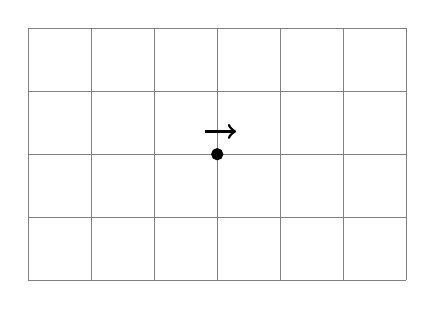
\begin{tikzpicture}[scale=0.8,x=1.0cm,y=1.0cm]
\draw [color=Gray, xstep=1.0cm,ystep=1.0cm] (-3.,-2.) grid (3.,2.);
\draw [->,color=black,line width=1.pt] (-0.2,0.3619794772370196) -- (0.3,0.3619794772370196);
\draw [fill=black] (0.,0.) circle (2.5pt);
\end{tikzpicture}


\end{minipage}\hfill
\begin{minipage}{0.32\textwidth}

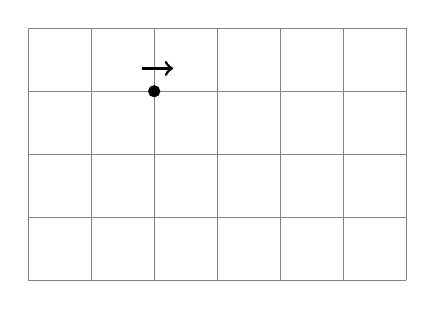
\begin{tikzpicture}[scale=0.8,x=1.0cm,y=1.0cm]
\draw [color=Gray, xstep=1.0cm,ystep=1.0cm] (-3.,-2.) grid (3.,2.);
\draw [->,color=black,line width=1.pt] (-1.2,1.3619794772370196) -- (-0.7,1.3619794772370196);
\draw [fill=black] (-1.,1.) circle (2.5pt);
\end{tikzpicture}

\end{minipage}\hfill
\begin{minipage}{0.32\textwidth}

 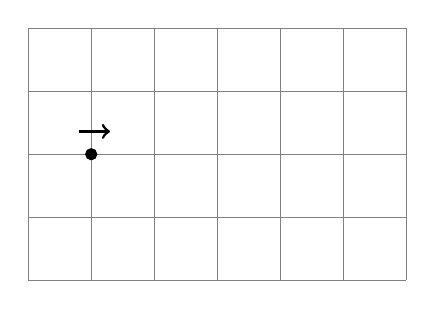
\begin{tikzpicture}[scale=0.8,x=1.0cm,y=1.0cm]
\draw [color=Gray, xstep=1.0cm,ystep=1.0cm] (-3.,-2.) grid (3.,2.);
\draw [->,color=black,line width=1.pt] (-2.2,0.3619794772370196) -- (-1.7,0.3619794772370196);
\draw [fill=black] (-2.,0.) circle (2.5pt);
\end{tikzpicture}

\end{minipage}%
\end{center}

\vfill

\setcounter{compteurinterro}{0}

\titreactif

\sautdeligne

%%%%%%%%%%%%%%%%
%%%% ÉNONCÉ %%%%
%%%%%%%%%%%%%%%%

  \begin{minipage}{0.48\textwidth}

    Dans cet exercice, on considère que chaque programme commence par les blocs ci-contre. Pour chaque programme, dessine la figure associée.

\end{minipage}\hfill
\begin{minipage}{0.48\textwidth}

    \fontsize{12}{0}\selectfont

    \begin{scratch}[scale=0.6,print]
        \blockinit{quand \greenflag est cliqué}
        \blockpen{stylo en position d'écriture}
        \blockmove{s’orienter à \ovalnum{90} degrés}
    \end{scratch}

\end{minipage}\hfill

\bigskip


\begin{minipage}{0.32\textwidth}

\begin{scratch}[scale=0.8,print]
	\blockmove{avancer de \ovalnum{10}}
	\blockrepeat{répéter \ovalnum{4} fois}
		{
		\blockmove{avancer de \ovalnum{20}}
		\blockmove{tourner \turnright{} de \ovalnum{90} degrés}
		}
	\blockmove{avancer de \ovalnum{10}}
\end{scratch}


\end{minipage}\hfill
\begin{minipage}{0.32\textwidth}

\begin{scratch}[scale=0.8,print]
	\blockrepeat{répéter \ovalnum{3} fois}
		{
		\blockmove{avancer de \ovalnum{10}}
		\blockmove{tourner \turnright{} de \ovalnum{90} degrés}
		\blockmove{avancer de \ovalnum{10}}
		\blockmove{tourner \turnleft{} de \ovalnum{90} degrés}
		}

\end{scratch}


\end{minipage}\hfill
\begin{minipage}{0.32\textwidth}

\begin{scratch}[scale=0.8,print]
\blockrepeat{répéter \ovalnum{5} fois}
{
     \blockrepeat{répéter \ovalnum{4} fois}
    {
    \blockmove{avancer de \ovalnum{10}}
    \blockmove{tourner \turnleft{} de \ovalnum{90} degrés}
    }
    \blockmove{avancer de \ovalnum{10}}
}
\end{scratch}


\end{minipage}%


\begin{center}
\begin{minipage}{0.32\textwidth}

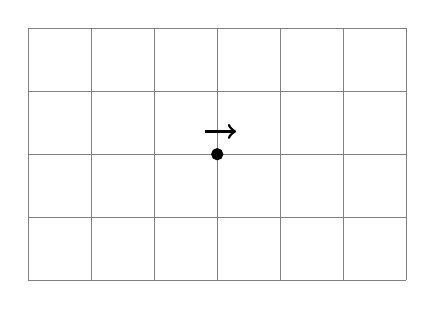
\begin{tikzpicture}[scale=0.8,x=1.0cm,y=1.0cm]
\draw [color=Gray, xstep=1.0cm,ystep=1.0cm] (-3.,-2.) grid (3.,2.);
\draw [->,color=black,line width=1.pt] (-0.2,0.3619794772370196) -- (0.3,0.3619794772370196);
\draw [fill=black] (0.,0.) circle (2.5pt);
\end{tikzpicture}


\end{minipage}\hfill
\begin{minipage}{0.32\textwidth}

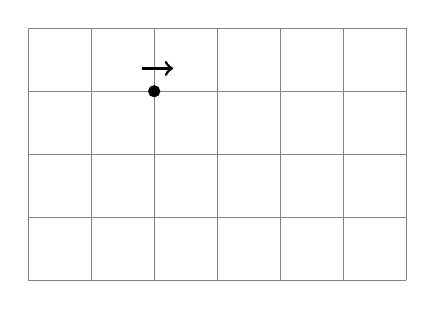
\begin{tikzpicture}[scale=0.8,x=1.0cm,y=1.0cm]
\draw [color=Gray, xstep=1.0cm,ystep=1.0cm] (-3.,-2.) grid (3.,2.);
\draw [->,color=black,line width=1.pt] (-1.2,1.3619794772370196) -- (-0.7,1.3619794772370196);
\draw [fill=black] (-1.,1.) circle (2.5pt);
\end{tikzpicture}

\end{minipage}\hfill
\begin{minipage}{0.32\textwidth}

 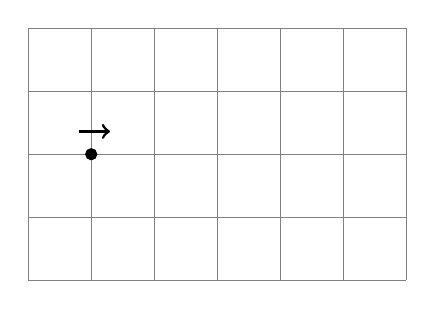
\begin{tikzpicture}[scale=0.8,x=1.0cm,y=1.0cm]
\draw [color=Gray, xstep=1.0cm,ystep=1.0cm] (-3.,-2.) grid (3.,2.);
\draw [->,color=black,line width=1.pt] (-2.2,0.3619794772370196) -- (-1.7,0.3619794772370196);
\draw [fill=black] (-2.,0.) circle (2.5pt);
\end{tikzpicture}

\end{minipage}%
\end{center}

\end{document}